\label{ch:fv}

\section{Discretization}

The physical systems we model are described by continuous mathematical
functions, $f(x,t)$ and their derivatives in space and time.  To
represent this continuous system on a computer we must discretize
it---convert the continuous function into a discrete number of points
in space at one or more discrete instances in time.
There are many different discretization methods used throughout the
physical sciences, engineering, and applied mathematics fields, each
with their own strengths and weaknesses.  Broadly speaking, we can
divide these methods into grid-based and gridless methods.

%% \begin{figure}[h]
%% \centering
%% 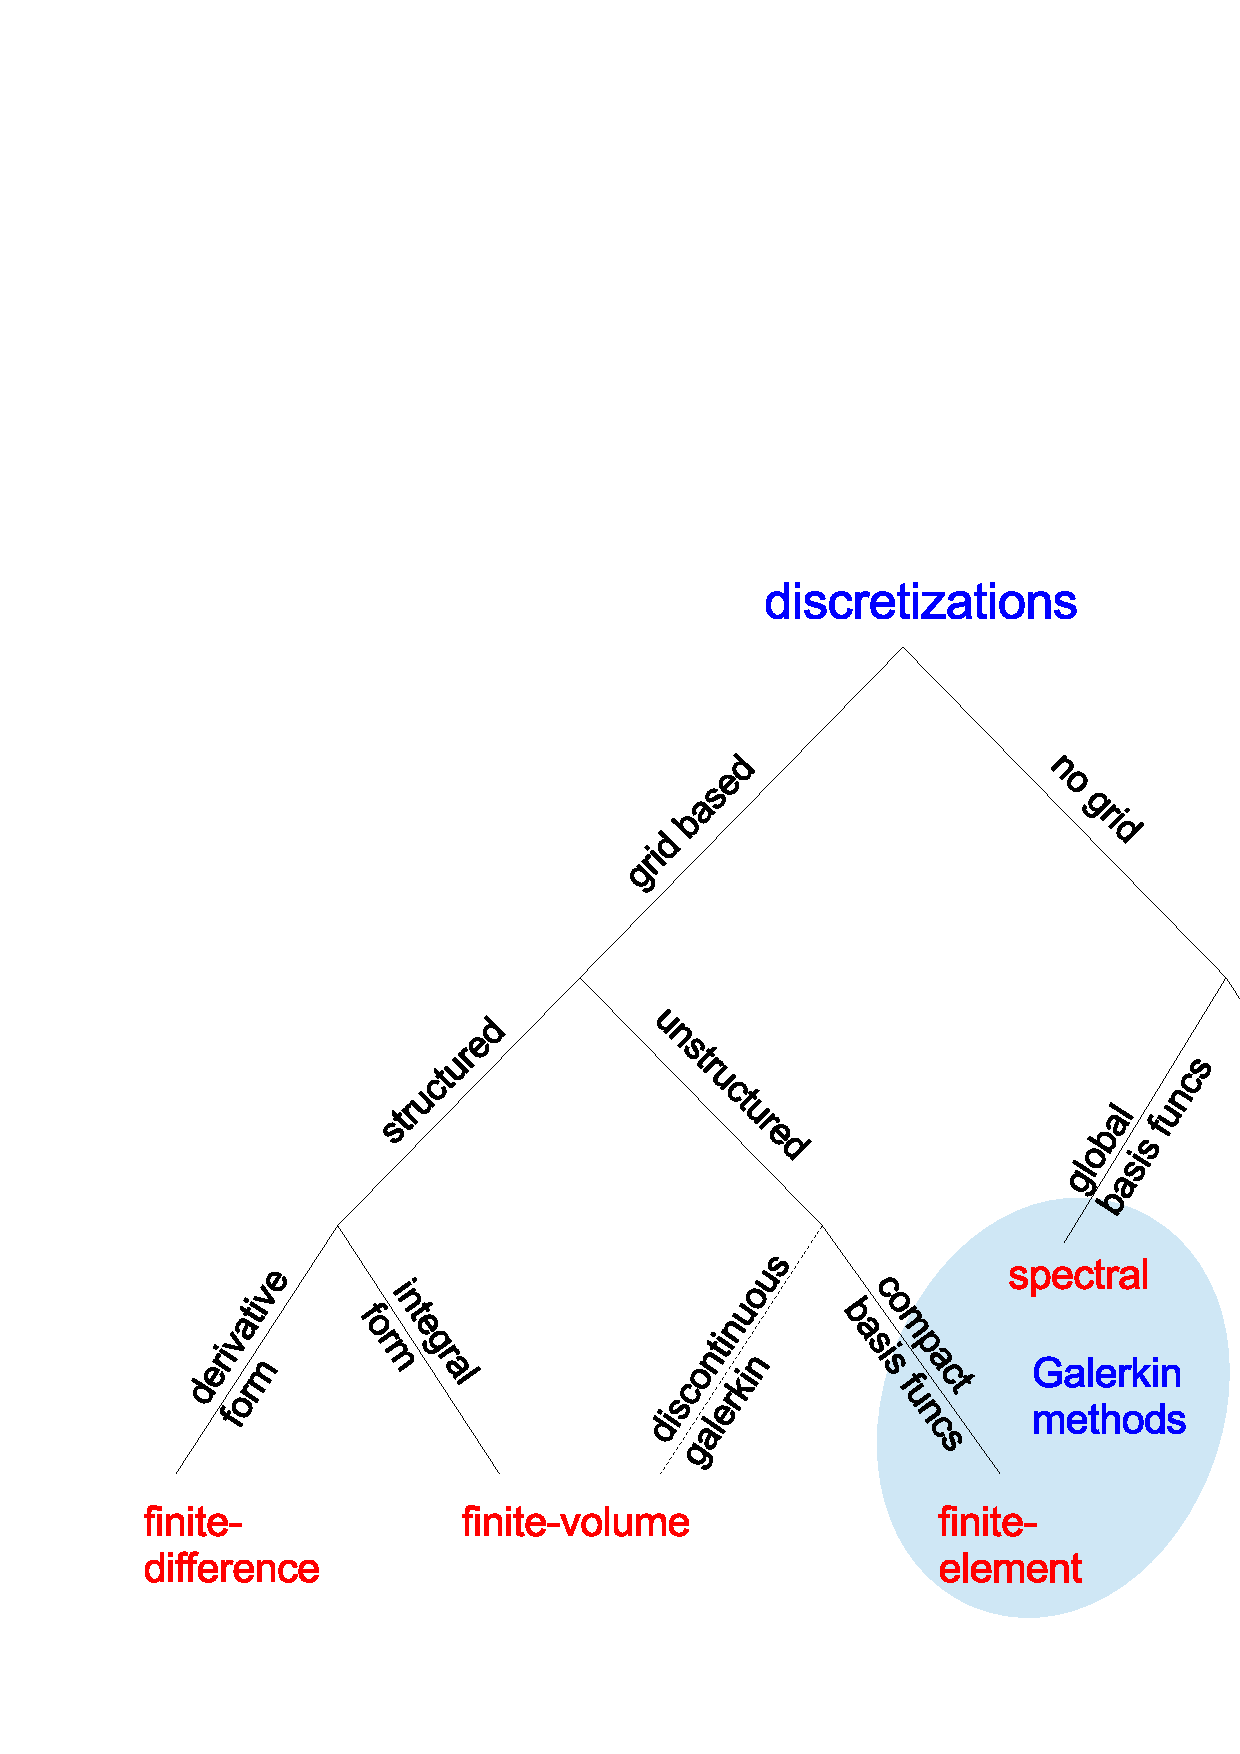
\includegraphics[width=\linewidth]{discretizations}
%% \caption[Taxonomy of different discretizations]
%%    {\label{fig:disc} Taxonomy of different discretizations.}
%% \end{figure}

Gridless methods include those which represent the function as a
superposition of continuous basis functions (e.g.\ sines and cosines).
This is the fundamental idea behind {\em spectral methods}.  A different
class of methods are those that use discrete particles to represent the
mass distribution and produce continuous functions by integrating
over these particles with a suitable kernel---this is the basis of
{\em smoothed particle hydrodynamics} (SPH)~\cite{SPH}.  SPH is a very popular
method in astrophysics.

For grid-based methods, we talk about both the style of the grid
(structured vs.\ unstructured) and the discretization method, e.g.\ the
finite-difference, finite-volume, and finite-element methods.

Structured grids are logically Cartesian.  This means that you can
reference the location of any cell in the computational domain via an
integer index in each spatial dimension.  From a programming
standpoint, the grid structure can be represented exactly by a
multi-dimensional array.  Unstructured grids don't have this simple
pattern.  A popular type of unstructured grid is created using
triangular cells (in 2-d) or tetrahedra (in 3-d).  \MarginPar{add
  figure} The main advantage of these grids is that you can easily
represent irregularly-shaped domains.  The disadvantage is that the
data structures required to describe the grid are more complicated
than a simple array (and tend to have more inefficient memory access).

\ifdefined\debugmode
Finite element methods are
widely used in engineering together with unstructured grids.  A type
of finite-element method called a {\em Galerkin method} can be formed
by integrating the continuous function against a compact basis set
represented by tetrahedra.  These methods work well with the irregular
geometries that arise in engineering.
\fi

Once a grid is established, the system of PDEs is converted into a
system of discrete equations on the grid.  Finite-difference and
finite-volume methods can both be applied to {\em structured grids}.
The main difference between these methods is that the
finite-difference methods build from the differential form of PDEs
while the finite-volume methods build from the integral form of the
PDEs.  The attractiveness of finite-volume methods is that
conservation is a natural consequence of the discretization---this is
why they are popular in astrophysics.

In these notes, we will focus on finite-volume techniques on
structured grids.


\section{Grid basics}

The grid is the fundamental object for representing continuous
functions in a discretized fashion, making them amenable to
computation.  In astrophysics, we typically use structured
grids---these are logically Cartesian, meaning that the position of a
quantity on the grid can be specified by a single integer index in
each dimension.  This works for our types of problems because
we don't have irregular geometries---we typically use boxes, disks,
or spheres.

We represent derivatives numerically by discretizing the domain into
a finite number of zones (a numerical grid).
This converts a continuous derivative into a difference of discrete data.
Different approximations have different levels of accuracy.

There are two main types of structured grids used in astrophysics:
{\em finite-difference} and {\em finite-volume}.  These differ in way
the data is represented.  On a finite-difference grid, the discrete
data is associated with a specific point in space.  On a
finite-volume grid, the discrete data is represented by averages over
a control volume.  Nevertheless, these methods can often lead to very
similar looking discrete equations.

Consider the set of grids show in Figure~\ref{fig:grids}.  On the top
is a classic finite-difference grid.  The discrete data, $f_i$, are
stored as points regularly spaced in $x$.  With this discretization,
the spatial locations of the points are simply $x_i = i \Delta x$,
where $i = 0, \ldots, N$\footnote{When you see $f_{i+1}$, you can
  think of this as meaning $f((i+1)\Delta x)$ or $f(x_i + \Delta x)$}.
Note that for a finite-sized domain, we would put a grid point
precisely on the physical boundary at each end.

The middle grid is also finite-difference, but now we imagine first
dividing the domain into $N$ cells or zones, and we store the discrete
data, $f_i$, at the center of the zone.  This is often called a {\em
  cell-centered finite-difference} grid.  The physical coordinate of
the zone centers (where the data lives) are: $x_i = (i + \myhalf)\Delta
x$, where $i = 0, \ldots, N-1$.  Note that now for a finite-sized
domain, the left edge of the first cell will be on the boundary and
the first data value will be associated at a point $\Delta x/2$ inside
the boundary.  A similar situation arises at the right physical
boundary.  Some finite-difference schemes stagger the variables,
e.g., putting velocity on the boundaries and density at the center.

Finally, the bottom grid is a finite-volume grid.  The layout looks
identical to the cell-centered finite difference grid, except now
instead of the discrete data being associated at a single point in
space, keep track of the total amount of $f$ in the zone (indicated as the shaded regions).  Since we generally don't know how $f$ varies in the zone,
we will typically talk about the average of $f$, $\favg{f}_i$, over
the zone, and represent this by a horizontal.  The total amount of $f$ in
the zone is then simply $\Delta x \favg{f}_i$. 
We label the left and right edges of a zone with half-integer indices
$i-\myhalf$ and $i+\myhalf$.  The physical coordinate of the center of the zone
is the same as in the cell-centered finite-difference case.


% the scripts to generate these figures are in figures/finite-volume
% as fd.py, ccfd.py, and fv.py
\begin{figure}[t]
\centering
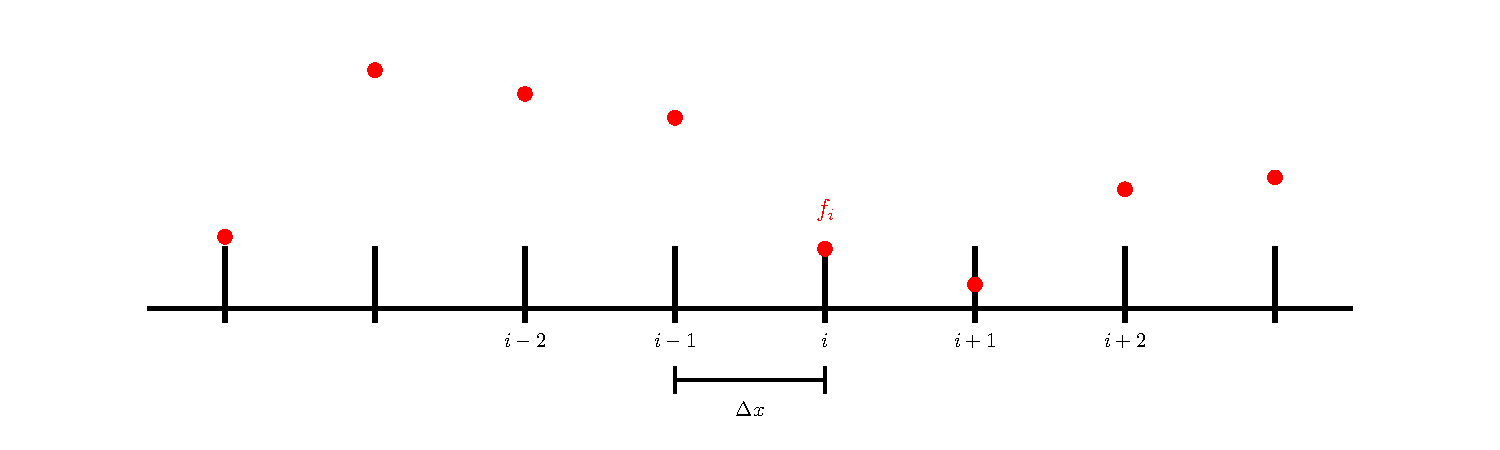
\includegraphics[width=\linewidth]{fd_grid} \\
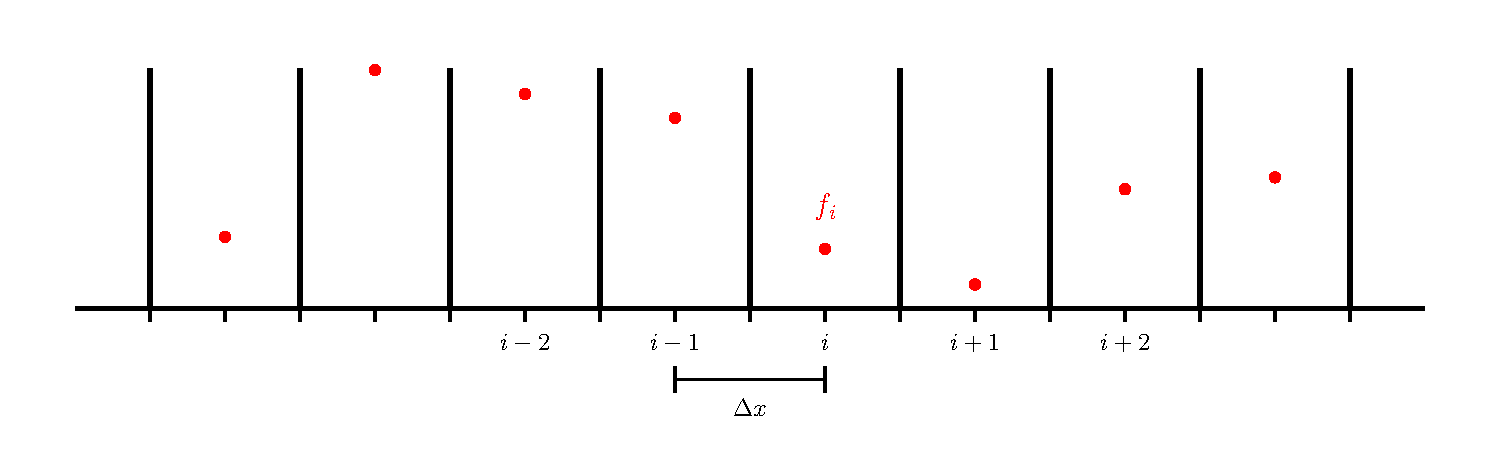
\includegraphics[width=\linewidth]{ccfd_grid} \\
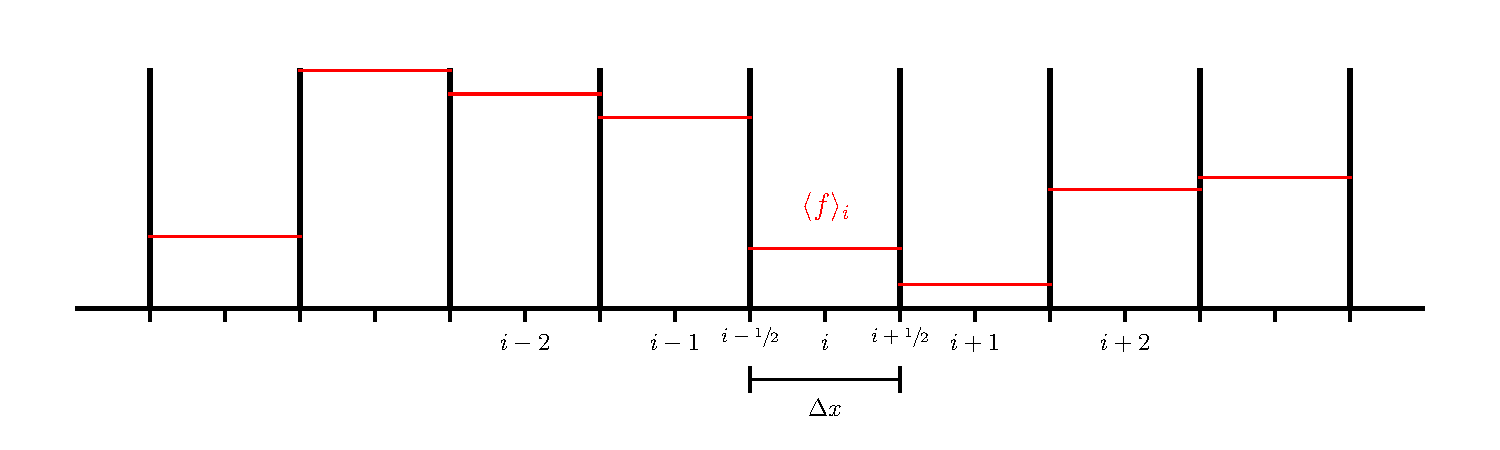
\includegraphics[width=\linewidth]{fv_grid}
\caption[Types of structured grids]{\label{fig:grids} Different types of structured grids showing
  the same data.  Top:
  a finite-difference grid---the discrete data are associated with a
  specific point in space.  Middle: a cell-centered finite-difference
  grid---again the data is at a specific point, but now we imagine the
  domain divided into zone with the data living at the center of each
  zone.  Bottom: a finite-volume grid---here the domain is divided
  into zones and we store the average value of the function within
  each zone.}
\end{figure}

In all cases, for a {\em regular} structured grid, we take $\Delta x$
to be constant.  For the finite-difference grids, the discrete value at
each point is obtained from the continuous function $f(x)$ as:
\begin{equation}
f_i = f(x_i)
\end{equation}


\section{Finite-volume grids}

In the finite-volume discretization, $f_i$ represents the average of
$f(x,t)$ over the interval $x_{i-\myhalf}$ to $x_{i+\myhalf}$, where
the half-integer indices denote the zone edges (i.e.\ $x_{i-\myhalf} =
x_i - \Delta x/2$):
\begin{equation}
\label{eq:fv_cc-a}
\favg{f}_i = \frac{1}{\Delta x} \int_{x_{i-\myhalf}}^{x_{i+\myhalf}} f(x) dx
\end{equation}
The lower panel of Figure~\ref{fig:grids} shows a finite-volume grid,
with the half-integer indices bounding zone $i$ marked.
%
% figure created with figures/finite-volume/simplegrid2.py
%% \begin{figure}[t]
%% \centering
%% 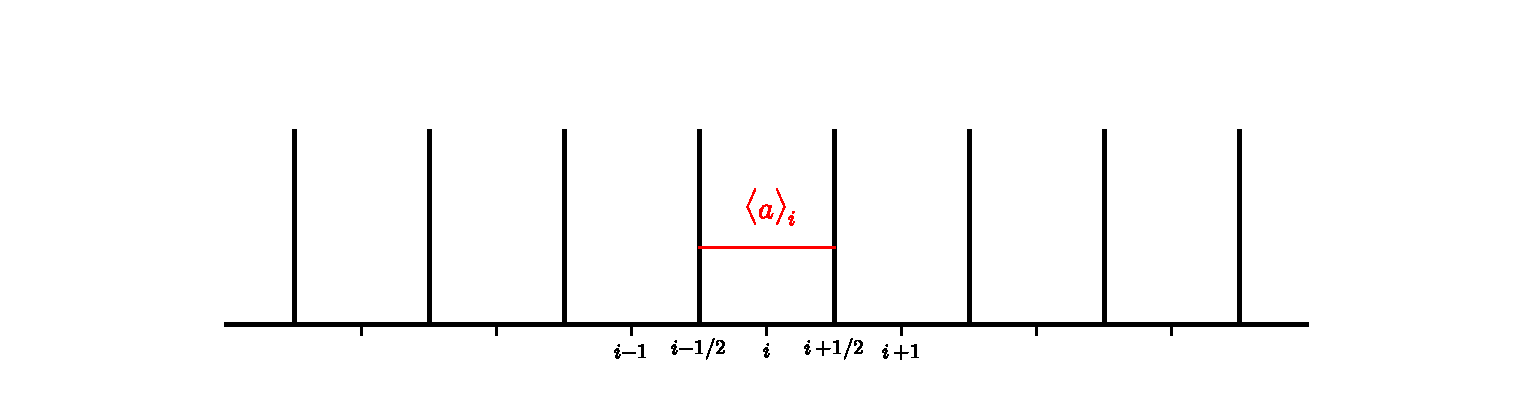
\includegraphics[width=\linewidth]{simplegrid2}
%% \caption[A simple 1-d finite-volume grid]{\label{fig:simplefv} A simple 1-d finite-volume
%%   grid with the zone-centered and zone-edge indexes.  Here we show
%%   only the data associated with zone $i$.}
%% \end{figure}
%
Here we've drawn $\favg{f}_i$ as a horizontal line spanning the entire zone---this
is to represent that it is an average within the volume defined by the zone
edges.
%
To second-order accuracy,
\begin{equation}
\label{eq:fv_cc}
\favg{f}_i = \frac{1}{\Delta x} \int_{x_{i-\myhalf}}^{x_{i+\myhalf}} f(x) dx \sim f(x_i)
\end{equation}

\begin{exercise}[Finite-volume vs.\ finite-difference centering]
{Show that Eq.~\ref{eq:fv_cc} is true to $O(\Delta x^2)$ by expanding
$f(x)$ as a Taylor series in the integral, e.g., as:
\begin{align}
f(x) = f(x_i) &+ f^\prime(x_i) (x - x_i) + \frac{1}{2} f^{\prime\prime}(x_i) (x - x_i)^2 \nonumber \\
%
 &+ \frac{1}{6} f^{\prime\prime\prime}(x_i) (x - x_i)^3 + \ldots
\end{align}
}
\end{exercise}

This means that we can treat the average of $f$ over a zone as simply
$f(x)$ evaluated at the zone center if we only want second-order
accuracy.  Using the subscript notation, we can express the average of
the zone to the right as $\favg{f}_{i+1}$.

When we want to interpolate data on a finite-volume grid, we want to
construct an interpolating polynomial that is conservative.  A {\em
  conservative interpolant} reconstructs a continuous functional form,
$f(x)$, from a collection of cell-averages subject to the requirement
that when $f(x)$ is averaged over a cell, it returns the original
cell-average.

\begin{exercise}[Conservative interpolation]
{\label{ex:consinterp}

Consider three cell averages: $\favg{f}_{i-1}$, $\favg{f}_{i}$, $\favg{f}_{i+1}$.  Fit a quadratic polynomial through these points,
 \begin{equation}
 f(x) = A (x - x_i)^2 + B (x - x_i) + C
 \end{equation}
 where the coefficients, $A$, $B$, and $C$ are found by applying the constraints:
 \begin{align}
 \favg{f}_{i-1} &= \frac{1}{\Delta x}
      \int_{x_{i-\mythreehalf}}^{x_{i-\myhalf}} f(x) dx \\
 \favg{f}_{i} &= \frac{1}{\Delta x}
      \int_{x_{i-\myhalf}}^{x_{i+\myhalf}} f(x) dx \\
 \favg{f}_{i+1} &= \frac{1}{\Delta x}
      \int_{x_{i+\myhalf}}^{x_{i+\mythreehalf}} f(x) dx
 \end{align}

Show that the conservative interpolant is:
\begin{align}
f(x) = &\frac{\favg{f}_{i-1} - 2 \favg{f}_i +
             \favg{f}_{i+1}}{2\Delta x^2} (x-x_i)^2 + \nonumber \\
       &\frac{\favg{f}_{i+1} - \favg{f}_{i-1}}
            {2\Delta x} (x-x_i) + \nonumber \\
       &\frac{-\favg{f}_{i-1} + 26 \favg{f}_i
             -\favg{f}_{i+1}}{24}
\end{align}
}
\end{exercise}

The {\sf Jupyter} notebook
\hydroexdoit{\href{https://github.com/zingale/hydro_examples/blob/master/finite-volume/conservative-interpolation.ipynb}{conservative-interpolation.ipynb}}
shows how to derive these interpolants using {\sf SymPy}, and gives
higher-order interpolants.


\subsection{Differences and order of accuracy}

In practice, when computing derivatives in a finite-volume
discretization, we can use the second-order centered difference from
\S~\ref{ch:intro:diff} treating the finite-volume data as living at the
cell-centers and still be second-order accurate.  For higher accuracy,
we can fit a {\em conservative interpolant} (as illustrated in
exercise~\ref{ex:consinterp}) to a collection of points and then
differentiate the interpolant itself.  \MarginPar{show convergence plot}

Notice that the righthand side of all derivative approximations involve
some linear combinations of $f_i$'s.  We call this the {\em stencil}.
The {\em width} of the stencil is a measure of how many zones on
either side of zone $i$ we reach when computing our approximation.

For example, a second derivative can be discretized as:
\begin{equation}
\left . \frac{d^2 f}{dx^2} \right |_i = \frac{f_{i+1} - 2 f_i + f_{i-1}}{\Delta x^2}
\end{equation}
The stencil on the righthand side encompasses 3 zones.

\subsection{Conservation}

The finite-volume grid is useful when dealing with conservation laws.
Consider the following system:
\begin{equation}
\frac{\partial \Uc}{\partial t} + \nabla \cdot \Fb(\Uc) = 0
\end{equation}
where $\Uc$ is a vector of conserved quantities and $\Fb(\Uc)$ is the flux
of each quantity.  This type of system arises, for example, in fluid
flow, where the system will represent conservation of mass, momentum,
and energy.

Consider one-dimension.
Integrating this system over a zone, and normalizing by $\Delta x$, we have:
\begin{equation}
\frac{1}{\Delta x} \int_{x_{i-\myhalf}}^{x_{i+\myhalf}} \ddt{\Uc} dx =
  -\frac{1}{\Delta x} \int_{x_{i-\myhalf}}^{x_{i+\myhalf}} \frac{\partial \Fb}{\partial x} dx
\end{equation}
On the left, we can take the time derivative out of the integral, and
we are left with the definition of a zone average, so this becomes
simply $\partial \favg{\Uc}_i/\partial t$.  On the right, we
apply the divergence theorem, giving:
\begin{equation}
\frac{\partial \favg{\Uc}_i}{\partial t} =
  - \frac{1}{\Delta x} \left \{ \left . \Fb(\Uc) \right |_{x_{i+\myhalf}} -
                                \left . \Fb(\Uc) \right |_{x_{i-\myhalf}} \right \}
\end{equation}
Independent of how we discretize in time, notice that we have the cell-average
on the left and that the righthand side
is simply a difference of fluxes through the interfaces of the zone.
For the $i+1$ zone, the update would be:
\begin{equation}
\label{eq:consup}
\frac{\partial \favg{\Uc}_{i+1}}{\partial t} =
  - \frac{1}{\Delta x} \left \{ \left . \Fb(\Uc) \right |_{x_{i+\mythreehalf}} -
                                \left . \Fb(\Uc) \right |_{x_{i+\myhalf}} \right \}
\end{equation}
Notice that this shares the flux at the $x_{i+\myhalf}$ interface, but with the
opposite sign.  \MarginPar{illustrate this} When all of the updates are done, the flux through each
boundary adds to one zone and subtracts from its neighbor, exactly conserving
(to round-off error) the quantity $\Uc$.  This cancellation of the sums
is an example of a {\em telescoping property}, and is the main reason
why finite-volume methods are attractive---conserved quantities are
conserved to machine (roundoff) precision.

Note that conservation is not the same as accuracy.  We can construct
the fluxes for our discretized equation by calling a random number
generator and we'd still be conservative, but not at all accurate.

\subsection{Boundary conditions with finite-volume grids}

\label{sec:fv:bcs}

Imagine that we wish to compute the derivative in every zone using:
\begin{equation}
\left . \frac{\partial f}{\partial x} \right |_i = \frac{f_i - f_{i-1}}{\Delta x} \enskip .
\label{eq:onesideddiff}
\end{equation}
If we denote the index corresponding to the leftmost zone in our
domain as `lo', then when we try to compute ${\partial f}/{\partial x}
|_\mathrm{lo}$, we will ``fall-off'' the grid, i.e., we need a value
of $f$ for zone $\mathrm{lo}-1$, which is outside the domain.  This is
where boundary conditions for our grid come into play.

We implement boundary conditions by extending the computational grid
beyond the physical domain (see Figure~\ref{fig:fv_gc}).  These
additional zones are called {\em ghost cells}.  They exist solely to
handle the boundary conditions and allow us to use the same update
equation (e.g.\ Eq.~\ref{eq:onesideddiff}) for all zones in the
domain.

% figure created with simplegrid-gc.py
\begin{figure}[t]
\centering
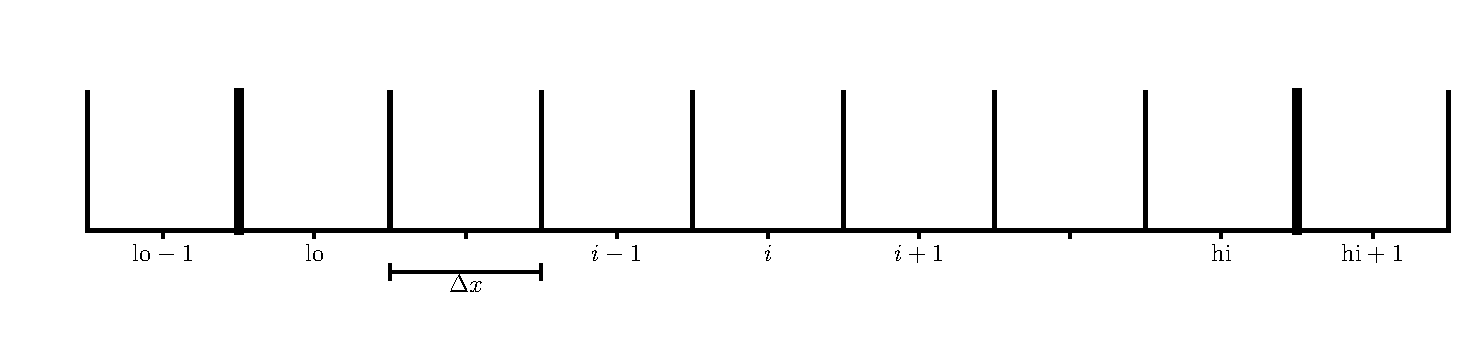
\includegraphics[width=\linewidth]{simplegrid_gc}
\caption[A simple 1-d finite-volume grid with ghost cells]
        {\label{fig:fv_gc} A simple 1-d finite-volume grid with a
          single ghost cell at each end of the domain.  The domain
          boundaries are indicated by the heavy vertical lines.  Here
          there are $\mathrm{hi}-\mathrm{lo}+1$ zones used in the
          discretization of the domain, with the first zone in the
          domain labeled $\mathrm{lo}$ and the last in the domain
          labeled $\mathrm{hi}$.}
\end{figure}

The number of ghostcells needed for the grid depends on how wide the
stencils used in the computation are.  The wider the stencil, the more
ghostcells are needed.

Periodic boundary conditions would be implemented as:
\begin{eqnarray}
f_{\mathrm{hi}+1} &=& f_\mathrm{lo} \\
f_{\mathrm{lo}-1} &=& f_\mathrm{hi}
\end{eqnarray}
A simple outflow (zero-gradient) boundary condition would be implemented as:
\begin{eqnarray}
f_{\mathrm{hi}+1} &=& f_\mathrm{hi} \\
f_{\mathrm{lo}-1} &=& f_\mathrm{lo}
\end{eqnarray}



\section{Going further}

\begin{itemize}

\item {\em Domain decomposition}: when running on a parallel computer,
 the work is divided up across processor using domain decomposition.
 Here, we break the computational domain into smaller sub-domains, and
 put one (or more) sub-domains on each processor.  Each sub-domain
 has its own perimeter of ghost cells.  These are now filled by copying
 information from the neighboring sub-domains or using the physical
 boundary conditions for the full domain, depending on where the
 ghost cells lie.  Figure~\ref{fig:domain} shows a simple decomposition of
 a domain into 6 sub-domains.

 % create with figures/finite-volume/domain.py
 \begin{figure}
 \centering
 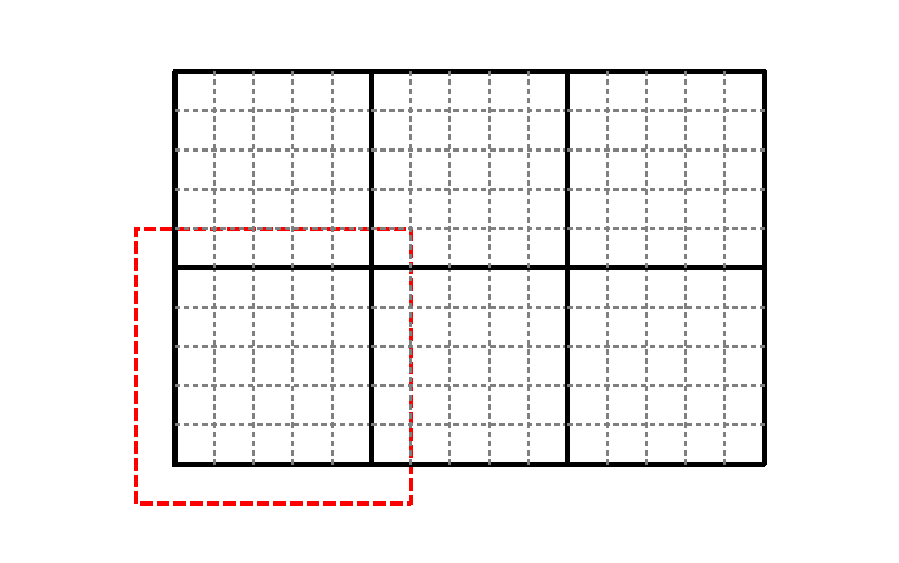
\includegraphics[width=\linewidth]{domain}
 \caption[Domain decomposition example] {\label{fig:domain} Domain
   decomposition of the computational domain into 6 separate
   sub-domains.  Each sub-domain here has $5\times 5$ zones.  For one
   of the sub-domains, the perimeter of ghost cells is illustrated as
   the red boundary.}
 \end{figure}

\item {\em AMR for structured grids}: adaptive mesh refinement uses a
  hierarchy of grids to focus resolution in regions of complex flow.
  For finite-volume codes, the standard reference for AMR is Berger \&
  Colella~\cite{berger-colella}.  Each level is an even integer
  multiple finer in resolution, and the grid cells line up with one
  another (i.e.\ in two-dimensions, four fine cells will be completely
  enclosed by a single coarse cell, when using a jump in resolution of
  2$\times$.)  This provides a natural way to enforce conservation.
  At coarse-fine interfaces, corrections are done to ensure
  consistency.

\item {\em Mapped grids}: mapped grids are (usually) logically
  Cartesian grids that use a function (map) to transform from
  a rectangular mesh (that corresponds to the array in memory)
  to a general curvilinear grid.  These maintain the performance
  characteristics of structured grids, since any zone can be
  directly indexed with an integer for each spatial dimension. \MarginPar{reference the Calhoun paper}

\item {\em Lagrangian grids}: a hybrid of particle and grid methods is
  provided by methods that move particles in a Lagrangian fashion and
  use a Voronoi tessellation of these particles to define the grid
  that finite-volume methods are applied to.  See, for example,
  the Arepo code paper~\cite{arepo}.
\end{itemize}
